\documentclass[a4paper, twocolumn, 10pt, revision]{ess}
\usepackage{dmsc}
\usepackage{paralist}
%\usepackage{esslogo}
\input{generated/revision}

\addbibresource{STAP-Reports.bib}

\newcommand{\pdfsubject}{Spectroscopy Scientific and Technical Advisory Panel}
\newcommand{\pdftitle}{Instrument Data Scientist Report}
\newcommand{\pdfauthor}{Gregory Tucker}
\newcommand{\pdfaffil}{European Spallation Source DMSC}
\hypersetup{%
  pdfinfo={%
    Title=\pdftitle,%
    Subject=\pdfsubject,%
    Author=\pdfauthor,%
    Revision=\revision,%
    Keywords={Revision:\revision,Affiliation:\pdfaffil}%
  }%
}

% set extra footer information
% \ifoot{\pdfauthor\\\pdfaffil}
% \ofoot{\pdftitle\\\revision}
% \cfoot{}


% \pagestyle{scrheadings}


\begin{document}
\titlehead{\pdfsubject \hfill Revision: \revision}
%\subject{\pdfsubject}
\title{\pdftitle}
\author{\pdfauthor}
\date{\revisiondate}
\maketitle

%\begin{abstract}
%This report represents a summary of work performed since October 2022.
%\end{abstract}

\section{Pixel mapping}
The last ESS Spectroscopy STAP Report \autocite{spectroscopy_stap_2022} included a request for information about pixel mapping plans.
%Interest was expressed about pixel mapping in the last ESS Spectroscopy STAP Report \autocite{spectroscopy_stap_2022}.

Comprehensive details are available from the Experiment Control and Data Curation (ECDC)
\href{https://confluence.esss.lu.se/display/ECDC/Instrument+Status+Overview}{Instrument Status Overview} page within 
ESS Confluence.
The CSPEC documentation there does not yet reflect the change to $^3$He detectors,
but should instead be similar to that for \href{https://project.esss.dk/owncloud/index.php/s/4M60TNdqkMcppUX}{BIFROST}.

A high-level summary of the planned pixelation scheme follows:
\begin{inparaenum}
\item signals from the ends of a wire, $A$ and $B$, are digitized by one of series of Front End Nodes;
\item a Readout Master collects the digitized signals, bundles them into packets along with timing information, and sends the packets to a server room located in the Central Utility Building, H01, on the ESS site;
\item an instance of the \href{https://github.com/ess-dmsc/event-formation-unit}{Event Formation Unit} (EFU) software uses linear charge division to pixelate each wire.
\end{inparaenum}

Conversion to pixels from the continuous charge-division signal, $x = A/(A+B)$, will require two values per tube to identify its ends.
The EFU extracts $x$ between the specified end-points and optionally applies a nonlinear correction with calibrated polynomial coefficients
before subdividing it into a configurable number of pixels.
The number of EFU pixels should match the position resolution of the tube.
%, and 100 pixels per tube are expected for BIFROST.
% -- in the case of BIFROST this is six values per wire due to the triple in-series tubes.

Since the ESS data transformation for spectroscopy will keep neutron event data and avoid unnecessarily producing histograms, 
combining pixels to, e.g., match instrumental resolution conditions, will only be performed preceding the final histogram-creating step.


\section{Project planning}
Since the October 2022 STAP meeting, extra emphasis has been placed on project planning at the IDS level.
As with other DMSC projects, a JIRA project,
\href{https://jira.esss.lu.se/projects/DMSCSPEC}{DMSC Spectroscopy},
has been created to track the DMSC deliverables for BIFROST and CSPEC.
Currently efforts are focused on aligning the project with requirements as seen by groups within DMSC as well as the BIFROST and CSPEC teams.


\section{Simulations}
Efforts to integrate McStas simulations into the ESS event pipeline continue \autocite{tucker_spectroscopy_stap_october_2022}.
Since the last report:
\begin{itemize}
\item The \href{https://github.com/g5t/mcstas-detector-tubes}{detector component}
      has been extended to support other arrangements of multiple $^3$He tubes,
      like the constant-radius MultiTube arrays now-expected for CSPEC.
      Figure \ref{fig:detector_tubes} shows multiple tube arrays now possible with the McStas component.
\item The \href{https://github.com/g5t/mcstas-readout-master}{readout master component}
      has been refactored. 
      The changes have made installing and using the shared library and McStas component easier on new systems,
      and allow for automatic EFU control even in parallel MPI runtime environments.
\item The full BIFROST spectrometer can now be used via McStasScript to simulate neutrons from the ESS source through to pixel identification in the EFU.
\item BIFROST primary spectrometer Monte Carlo Particle List (MCPL) files exist for a small subset of possible chopper settings,
      which can be used to significantly improve the simulated instrument throughput with, e.g., complex Union samples.
\end{itemize}

Planned next-steps include:
\begin{itemize}
	\item \href{https://jira.esss.lu.se/projects/DMSCSPEC/issues/DMSCSPEC-8}{\texttt{DMSCSPEC-8}}
		Complete the readout chain by getting simulated events from the EFU through to a NeXus file.
	\item \href{https://jira.esss.lu.se/projects/DMSCSPEC/issues/DMSCSPEC-9}{\texttt{DMSCSPEC-9}}
		Simulate a BIFROST experimenti, including produing at least one $\QvecE$ map.
	\item \href{https://jira.esss.lu.se/projects/DMSCSPEC/issues/DMSCSPEC-10}{\texttt{DMSCSPEC-10}}
		Pass the simulated experiment data through the data transformation workflow.
\end{itemize}

\begin{figure}
\begin{centering}
	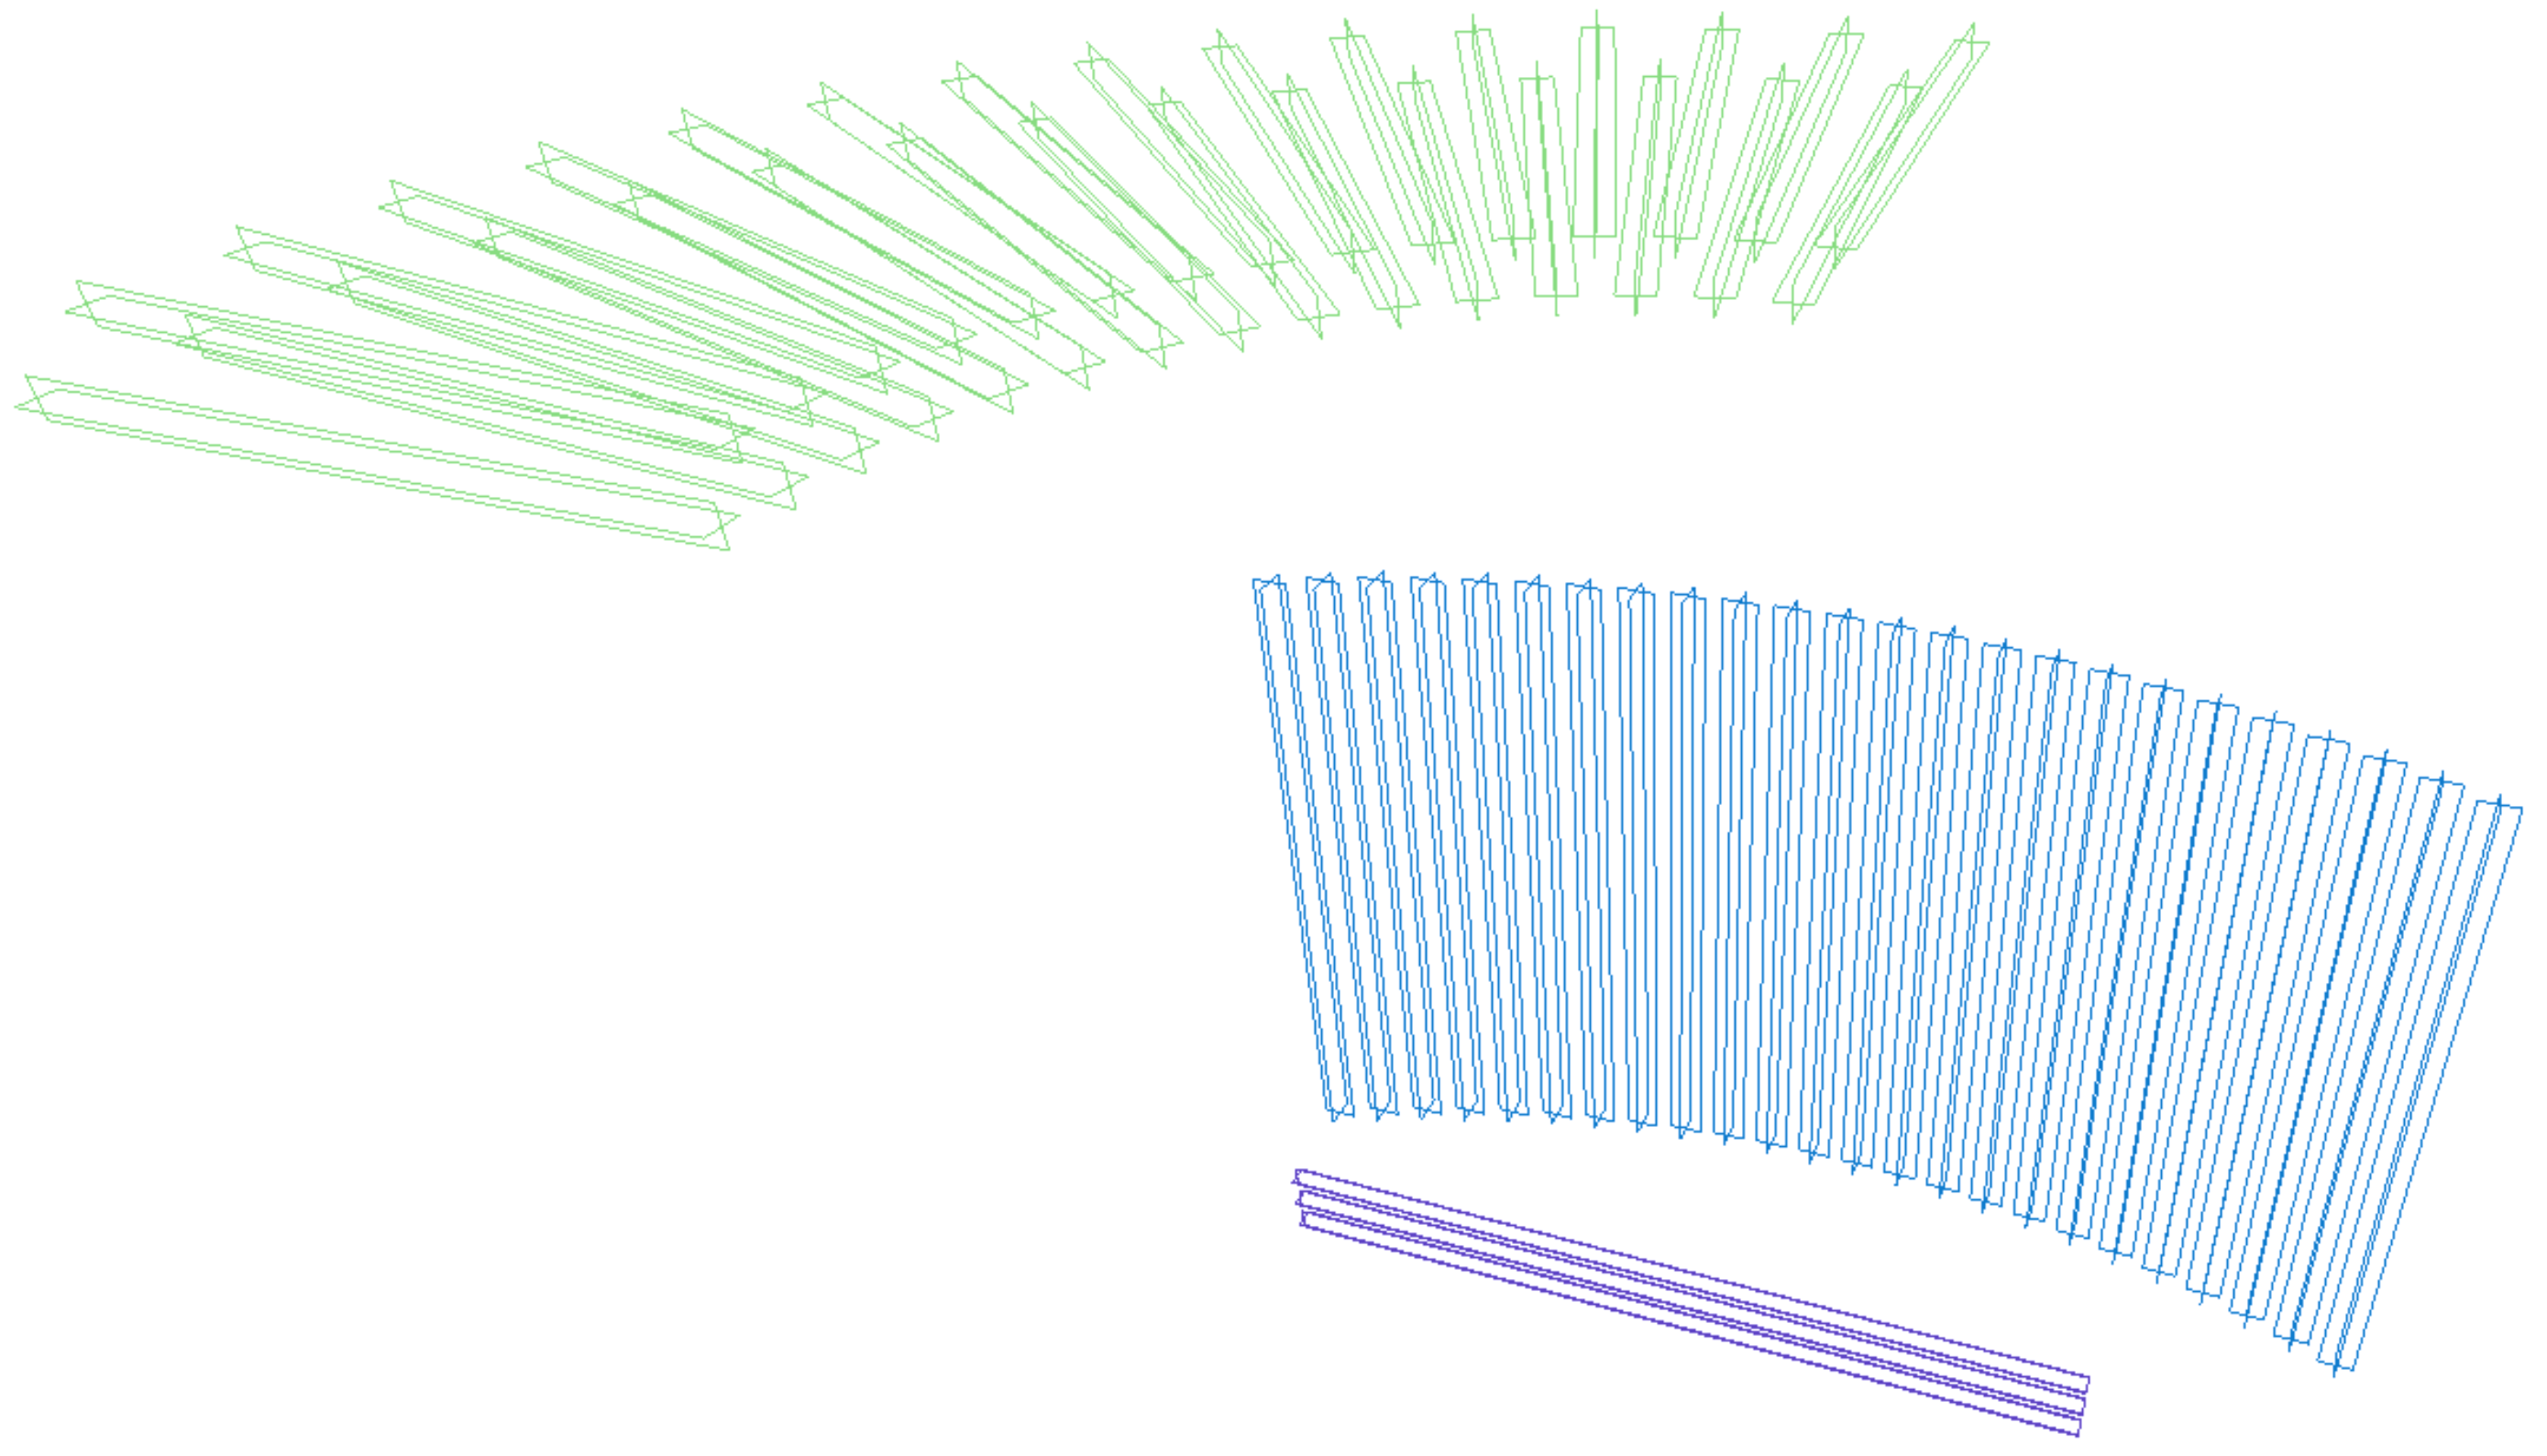
\includegraphics[width=\columnwidth]{detector_tubes}
\end{centering}
\caption{%
Multiple tube arrays in a test McStas instrument, including a BIFROST triplet (purple);
	a curved array (blue), like those planned for CSPEC but much shorter to fit in this image;
	a double-layer fan array (green), like that used on CAMEA.
\label{fig:detector_tubes}}
\end{figure}


\section{Flexible user tools}
%It is undoubtable that 
Some tasks are made easier through graphical user interfaces (GUI) to scripts or other routines.
A user may request a tool to help carry out a measurement, which must be flexible enough to support their specific use case,
and must be available quickly if it is to be useful.

Python is the language of choice for all ESS software interfaces since it is free, open source, and has an
extensive catalog of community-provided modules to augment its capabilities.
These qualities make it well suited to rapid prototyping and development,
which in turn makes it an ideal language for producing user-facing tools. %,
%especially ones which should interact with other ESS programs.

Thanks to the vast module catalog, there are many options for graphical interfaces in Python.
One option that requires little development effort to use in simple GUIs is
\href{https://ipywidgets.readthedocs.io/}{Jupyter Widgets}
which provide graphical interfaces to
\href{https://jupyter.org/}{Jupyter} notebooks.
Previously the use of \href{https://voila.readthedocs.io/}{voila} has been discussed for stand-alone GUIs \autocite{tucker_spectroscopy_stap_april_2022}.

To make any GUI tool written in Python available to users we can 
\begin{inparaenum}
\item distribute installers,
\item host it on ESS hardware,
\item distribute source files, or
\item make use of client-side web browser based interfaces.
\end{inparaenum}

% Distributed installers
Producing and distributing installers for any application can be resource intensive.
Such an investment may be worthwhile for large stable programs or performance sensitive applications,
but is likely wasteful for user tools.

% Host on ESS hardware
Hosting on ESS hardware can reduce a large part of the development effort compared to distributing installers;
mainly from having machine control and only targeting a single machine (or multiple identical machines).
%One option is to install the tool within a VISA virtual-machine instance,
%another is to host the tool as part of a website.
%Both of these options still require relatively high resource investments, which may not be suitable for in-development user tools.
Still, configuring and running the hosting system requires relatively high resource use,
which may not be suitable for in-development user tools.

% Tutorials + automated environment setup
Distributing the source files which constitute a Python tool confers all of the advantages of open-source software.
There may exist a high entry-barrier, however, since Python's modularity can make it challenging to use code written on another machine due to differing computing environments.
Semi-automatic configuration of computing environments is possible via a variety of tools, notably
\href{https://github.com/conda-forge/miniforge}{mamba},
but as they require installation and subsequent command-line use they may not be suitable for all users.

% WebAssembly
Web browser based interfaces have the significant advantage that they run on top of software which is almost-certainly
already present on a user's computer.
Through WebAssembly and the \href{https://pyodide.org/}{Pyodide} Python distribution it is possible
to run Python-based tools on a user's machine with no user-configuration and near-native performace.
It is even possible to run notebooks in a user's browser via \href{https://jupyterlite.readthedocs.io/}{Jupyterlite}.
For simple GUI tools this can allow for both rapid development and ease of use, even for novice users.

Recently, to support design of a new magnet a tool was required to help visualize the effect different opening-angles would have on accessible reciprocal space
for a direct-geometry spectrometer (DGS) like CSPEC.
The intended audience for the tool were the engineers, technicians, and scientists involved in setting the magnet design criteria,
but similar tool could prove useful for \emph{users} of a magnet on a DGS as well.
The source code of the tool is hosted on
\href{https://github.com/g5t/tof-tools/}{Github}
which also provides free webhosting for the
\href{https://g5t.github.io/tof-tools/lab?path=accessible.ipynb}{Jupyterlite interface}.
The tool running after interacting with some of the GUI elements is shown in figure \ref{fig:tof-tool}.

\begin{figure}
\begin{centering}
	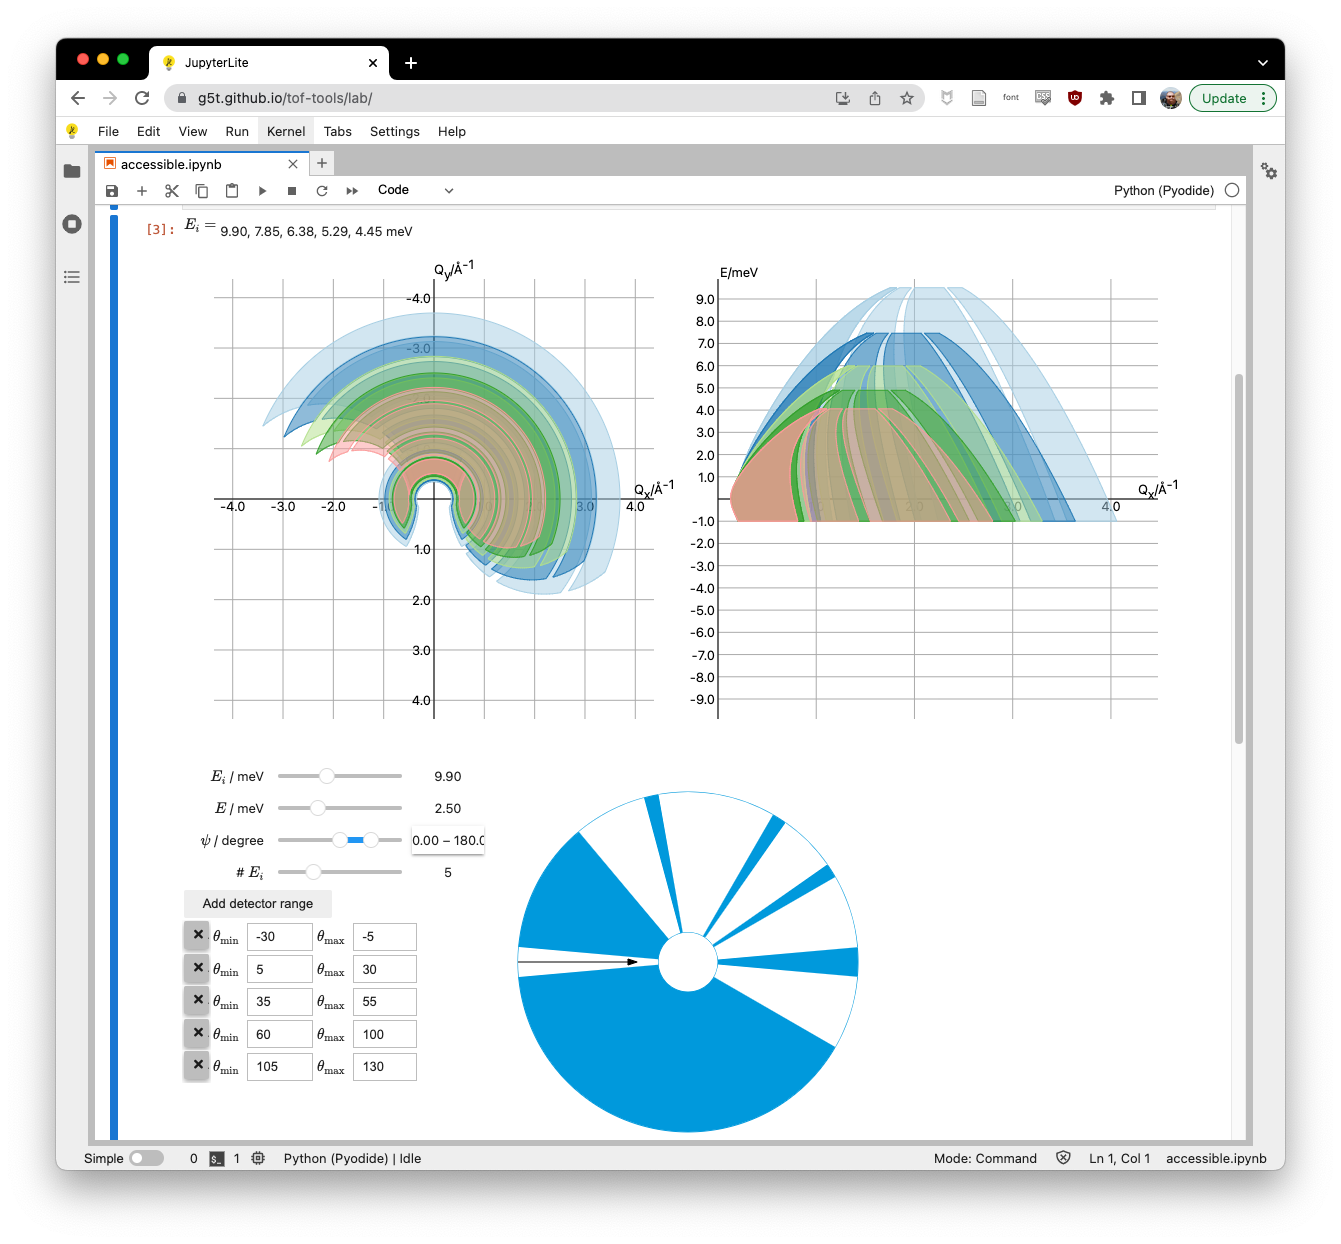
\includegraphics[width=\columnwidth]{tof-tool}
\end{centering}
\caption{The magnet opening-angle visualization tool, running in a Jupyterlite notebook. \label{fig:tof-tool}}
\end{figure}






\printbibliography
\end{document}
